\documentclass[12pt]{article}

\usepackage[utf8]{inputenc}
\usepackage[T1]{fontenc}
\usepackage{amssymb}
\usepackage{amsmath}
\usepackage{geometry}
\usepackage{parskip}
\usepackage{setspace}
\usepackage{graphicx}
\usepackage{hyperref}
\usepackage{indentfirst}
\usepackage{booktabs}
\usepackage{multirow}

\geometry{a4paper, margin=1in}
\onehalfspacing{}
\setlength{\parindent}{2em}
\setlength{\parskip}{0.5\baselineskip}

\title{A study on the Detection of Gender Antagonism Tendency in Chinese Social Media Based on CMLG Model}
\author{%
Author: \underline{Yonghao Yang} \\
Institution/School: \underline{Wuhan University} \\
Email: \underline{13235595638@163.com}%
}
\date{\today}

\begin{document}

\maketitle

\begin{abstract}
Gender-antagonistic discourse pervades Chinese social media, yet automatic detection remains unreliable due to the informal register, creative character-play, and noisy human annotations typical of this domain. We propose CMLG, a model that fuses CKBERT contextual embeddings, BGE dense embeddings, pinyin phonetic vectors, and wubi structural vectors through learnable feature-level attention, and classifies the fused sequence with a Bi-GRU backbone. To address label noise---which we identify as the dominant performance bottleneck---we introduce a cleaning pipeline in which three heterogeneous LLMs (Qwen2.5-72B, GLM-4-32B, DeepSeek-V3) independently vote on every sample. Ablation across five feature configurations and three dataset versions (original, majority-vote cleaned, unanimous-agreement cleaned) reveals two key findings: (1) label cleaning raises macro F1 from 0.7824 to 0.9007 (+12pp), an effect that also holds for SVM and BERT baselines (9--14pp gains); (2) Chinese-specific orthographic features (pinyin, wubi) are ineffective on noisy labels but become the strongest configuration once labels are cleaned, indicating that annotation quality gates the learnability of fine-grained linguistic cues.
\end{abstract}

\noindent\textbf{Keywords:} gender antagonism; deep learning; LLM-assisted data cleaning; feature-level attention fusion; Chinese NLP

\section{Introduction}
Gender-oriented hostility on social media has become a pressing societal concern [1,2], with documented effects on the psychological well-being of younger cohorts [2] and broader links to rising domestic tensions and declining willingness to marry or bear children [2,3]. Despite this, reliable automatic detection methods for Chinese-language platforms remain scarce. English-language sexism detection has seen steady progress in both benchmarks and modeling [4--7,16,17], but Chinese online discourse poses additional challenges: homophonic substitution, shape-similar character-play, and other creative evasion tactics that standard NLP pipelines cannot easily handle [9].

We define ``gender antagonism tendency'' as the directional stance an expression conveys toward a gender group, rather than its hostility intensity alone [2]. Although a three-class formulation (pro-male/anti-female, pro-female/anti-male, neutral) was initially planned, the available SWSR corpus [8] supplies only binary labels, and preliminary trials showed that current LLMs can exhibit gender biases that make them unsuitable as sole annotators for fine-grained directional labeling. We therefore work with a binary task---gender-antagonistic (label~1) vs.\ neutral (label~0)---and leave directional classification for future work.

This study makes three contributions. First, we design CMLG (CKBERT-based Multi-feature LLM-enhanced Bi-GRU), which fuses CKBERT contextual embeddings, BGE dense embeddings, pinyin phonetic vectors, and wubi structural vectors through learnable attention, combining pretrained semantics with Chinese-specific orthographic cues. Second, we build an LLM-assisted data cleaning pipeline based on three-model majority voting, producing two re-labeled dataset variants that enable controlled study of how label quality affects classification. Third, through ablation experiments spanning three dataset versions, five feature configurations, and two baselines, we show that label quality---not model architecture or feature engineering---is the dominant factor, and that Chinese orthographic features shift from useless to most valuable once annotation noise is removed.

\section{Related Work}

\subsection{Gender Hostility and Hate Speech Detection}
Gender-based hostility detection spans dataset construction and modeling advances. Gutam et al.\ [4] coupled BERT with community-enhanced annotations and reduced manual moderation workload by 40\%; Singh et al.\ [5] built the first Hindi--English code-mixed misogyny benchmark, with mBERT performing best. On the modeling side, Vivekananda et al.\ [6] explored BERT--classical-ML hybrids with weak supervision, while Mohasseb et al.\ [7] combined LDA with Sentence-Transformers for data augmentation, focusing on cross-corpus transfer. The broader hate speech literature [16] and the offensive-vs.-hateful distinction studied by Davidson et al.\ [17] are also relevant, as the boundary between antagonistic and merely blunt gender-related speech presents a similar challenge in our setting.

\subsection{Chinese-language Research}
Chinese-language efforts in this area remain limited. Jiang et al.\ [8] released SWSR, the first Chinese corpus annotated for online sexism at three granularities (binary, type, target). Ma et al.\ [9] augmented SWSR with pictographic and structural character features and reported a 5.19pp F1 gain. Sun et al.\ [18] investigated BERT fine-tuning strategies for Chinese text classification across multiple benchmarks. Our work extends this line by introducing a multi-stream architecture that separates phonetic, structural, and semantic channels, and by coupling it with LLM-based label cleaning.

\subsection{Label Noise in Supervised Learning}
Noisy labels are a pervasive problem in text classification, especially with crowdsourced annotations. Fr\'{e}nay and Verleysen [19] survey classical approaches---noise modeling, sample filtering, and robust loss design. Song et al.\ [20] cover deep-learning-specific techniques including sample re-weighting and meta-learning. Our pipeline takes the filtering route: rather than designing a noise-tolerant learner, we use multi-LLM consensus to correct labels before training.

\section{Methodology}

\subsection{Dataset}

\subsubsection{Data Source and Problem Formulation}
We use the SWSR dataset [8], retaining the \texttt{comment\_text} and \texttt{label} columns. The corpus contains 8{,}969 samples: 5{,}876 gender-neutral (label~0, 65.5\%) and 3{,}093 gender-antagonistic (label~1, 34.5\%). The task is binary text classification.

\subsubsection{LLM-Assisted Label Cleaning}
\label{sec:llm-cleaning}
To quantify and reduce annotation noise, we designed a cleaning pipeline based on three-model majority voting. Three LLMs---Qwen2.5-72B-Instruct, GLM-4-32B-0414, and DeepSeek-V3---each independently classify every sample using a structured Chinese prompt (Appendix~A). Predictions are aggregated by majority rule, yielding two cleaned variants:

\begin{itemize}
    \item \textbf{Cleaned-Full} (8{,}962 samples): all samples with a valid majority vote, relabeled accordingly. The label distribution shifts to 5{,}419 neutral (60.5\%) and 3{,}543 opposing (39.5\%).
    \item \textbf{Cleaned-HighConf} (6{,}793 samples): only samples where all three models unanimously agree, providing the highest label confidence. The distribution is 4{,}219 neutral (62.1\%) and 2{,}574 opposing (37.9\%).
\end{itemize}

Comparing original and cleaned labels, roughly 18.3\% of the original annotations disagree with the LLM consensus---a non-trivial noise rate. Table~\ref{tab:llm-stats} reports the per-model statistics.

\begin{table}[htbp]
\centering
\caption{Per-LLM cleaning statistics on the full 8{,}969-sample corpus.}
\label{tab:llm-stats}
\begin{tabular}{lccc}
\toprule
 & Qwen2.5-72B & GLM-4-32B & DeepSeek-V3 \\
\midrule
Valid responses & 87.4\% & 99.5\% & 99.5\% \\
Agreement w/ original labels & 75.3\% & 80.2\% & 81.5\% \\
Agreement w/ majority vote & 87.4\% & 96.1\% & 90.6\% \\
\midrule
Pairwise agreement & \multicolumn{3}{c}{Qwen--GLM: 84.5\%, Qwen--DS: 77.0\%, GLM--DS: 86.7\%} \\
Unanimous agreement & \multicolumn{3}{c}{6{,}793 / 8{,}969 samples (75.7\%)} \\
\bottomrule
\end{tabular}
\end{table}

\subsection{Feature Extraction}
Four parallel streams capture complementary aspects of each input text. Table~\ref{tab:features} summarizes the streams.

\begin{table}[htbp]
\centering
\caption{Feature streams used in CMLG.}
\label{tab:features}
\begin{tabular}{lllp{5.8cm}}
\toprule
Stream & Encoder & Dim & Rationale \\
\midrule
CKBERT ($v_c$) & CK-BERT [10,12] & $T \times 1024$ & Knowledge-enhanced contextual embeddings; primary semantic channel. \\
BGE ($v_b$) & BGE-base-zh-v1.5 [13] & $T \times 768$ & Dense sentence-level semantics from a separate pretraining objective. \\
Pinyin ($v_p$) & Word2Vec [14] & $T \times 256$ & Captures homophonic substitution (e.g., swapping sensitive words for characters that sound alike). \\
Wubi ($v_w$) & Word2Vec [14] & $T \times 256$ & Captures shape-similar character substitution via Wubi keystroke sequences. \\
\bottomrule
\end{tabular}
\end{table}

For CKBERT and BGE, character-level embeddings are recovered through offset mapping; where a subword token spans multiple characters, embeddings are averaged. Pinyin and wubi Word2Vec models are trained on the corpus itself and L2-normalized per token. CKBERT and BGE embeddings are extracted once and cached; pinyin and wubi models are retrained per dataset variant to reflect corpus composition differences.

\subsection{Feature-Level Attention Fusion}
\label{sec:attention-fusion}
The four streams differ in dimensionality (1024, 768, 256, 256); naively concatenating them would let higher-dimensional streams dominate gradient updates. We address this with a two-stage fusion.

\textbf{Stage 1: Per-stream Projection.} Each stream $v_k$ ($k \in \{c, p, w, b\}$) is projected to a common dimensionality $d = 128$ via a learnable linear layer, Layer Normalization, and GELU activation:
\[
\hat{v}_k = \mathrm{GELU}\bigl(\mathrm{LayerNorm}(W_k \, v_k + b_k)\bigr), \quad \hat{v}_k \in \mathbb{R}^{T \times 128}
\]
where $W_k \in \mathbb{R}^{128 \times d_k}$ is the projection matrix for stream $k$ with original dimensionality $d_k$, and $b_k \in \mathbb{R}^{128}$ is the bias.

\textbf{Stage 2: Additive Attention.} Following Bahdanau et al.\ [15], we compute a scalar attention score for each stream at each character position $t$. The $K$ projected features ($K$ = number of active streams) are stacked into $\mathbf{H} \in \mathbb{R}^{T \times K \times 128}$, and attention weights are:
\[
\alpha_{t,k} = \frac{\exp\bigl(\mathbf{v}^\top \tanh(\mathbf{W}_a \, \hat{v}_{t,k})\bigr)}{\sum_{j=1}^{K} \exp\bigl(\mathbf{v}^\top \tanh(\mathbf{W}_a \, \hat{v}_{t,j})\bigr)}
\]
where $\mathbf{W}_a \in \mathbb{R}^{128 \times 128}$ is a learnable weight matrix and $\mathbf{v} \in \mathbb{R}^{128}$ is a learnable context vector. The fused representation is:
\[
v_t^{\mathrm{fused}} = \sum_{k=1}^{K} \alpha_{t,k} \, \hat{v}_{t,k} \in \mathbb{R}^{128}
\]
This lets the network emphasize whichever stream is most informative at each character position, rather than applying a fixed weighting.

\subsection{Classification Network}
Figure~\ref{fig:architecture} illustrates the full CMLG pipeline.

\begin{figure}[htbp]
\centering
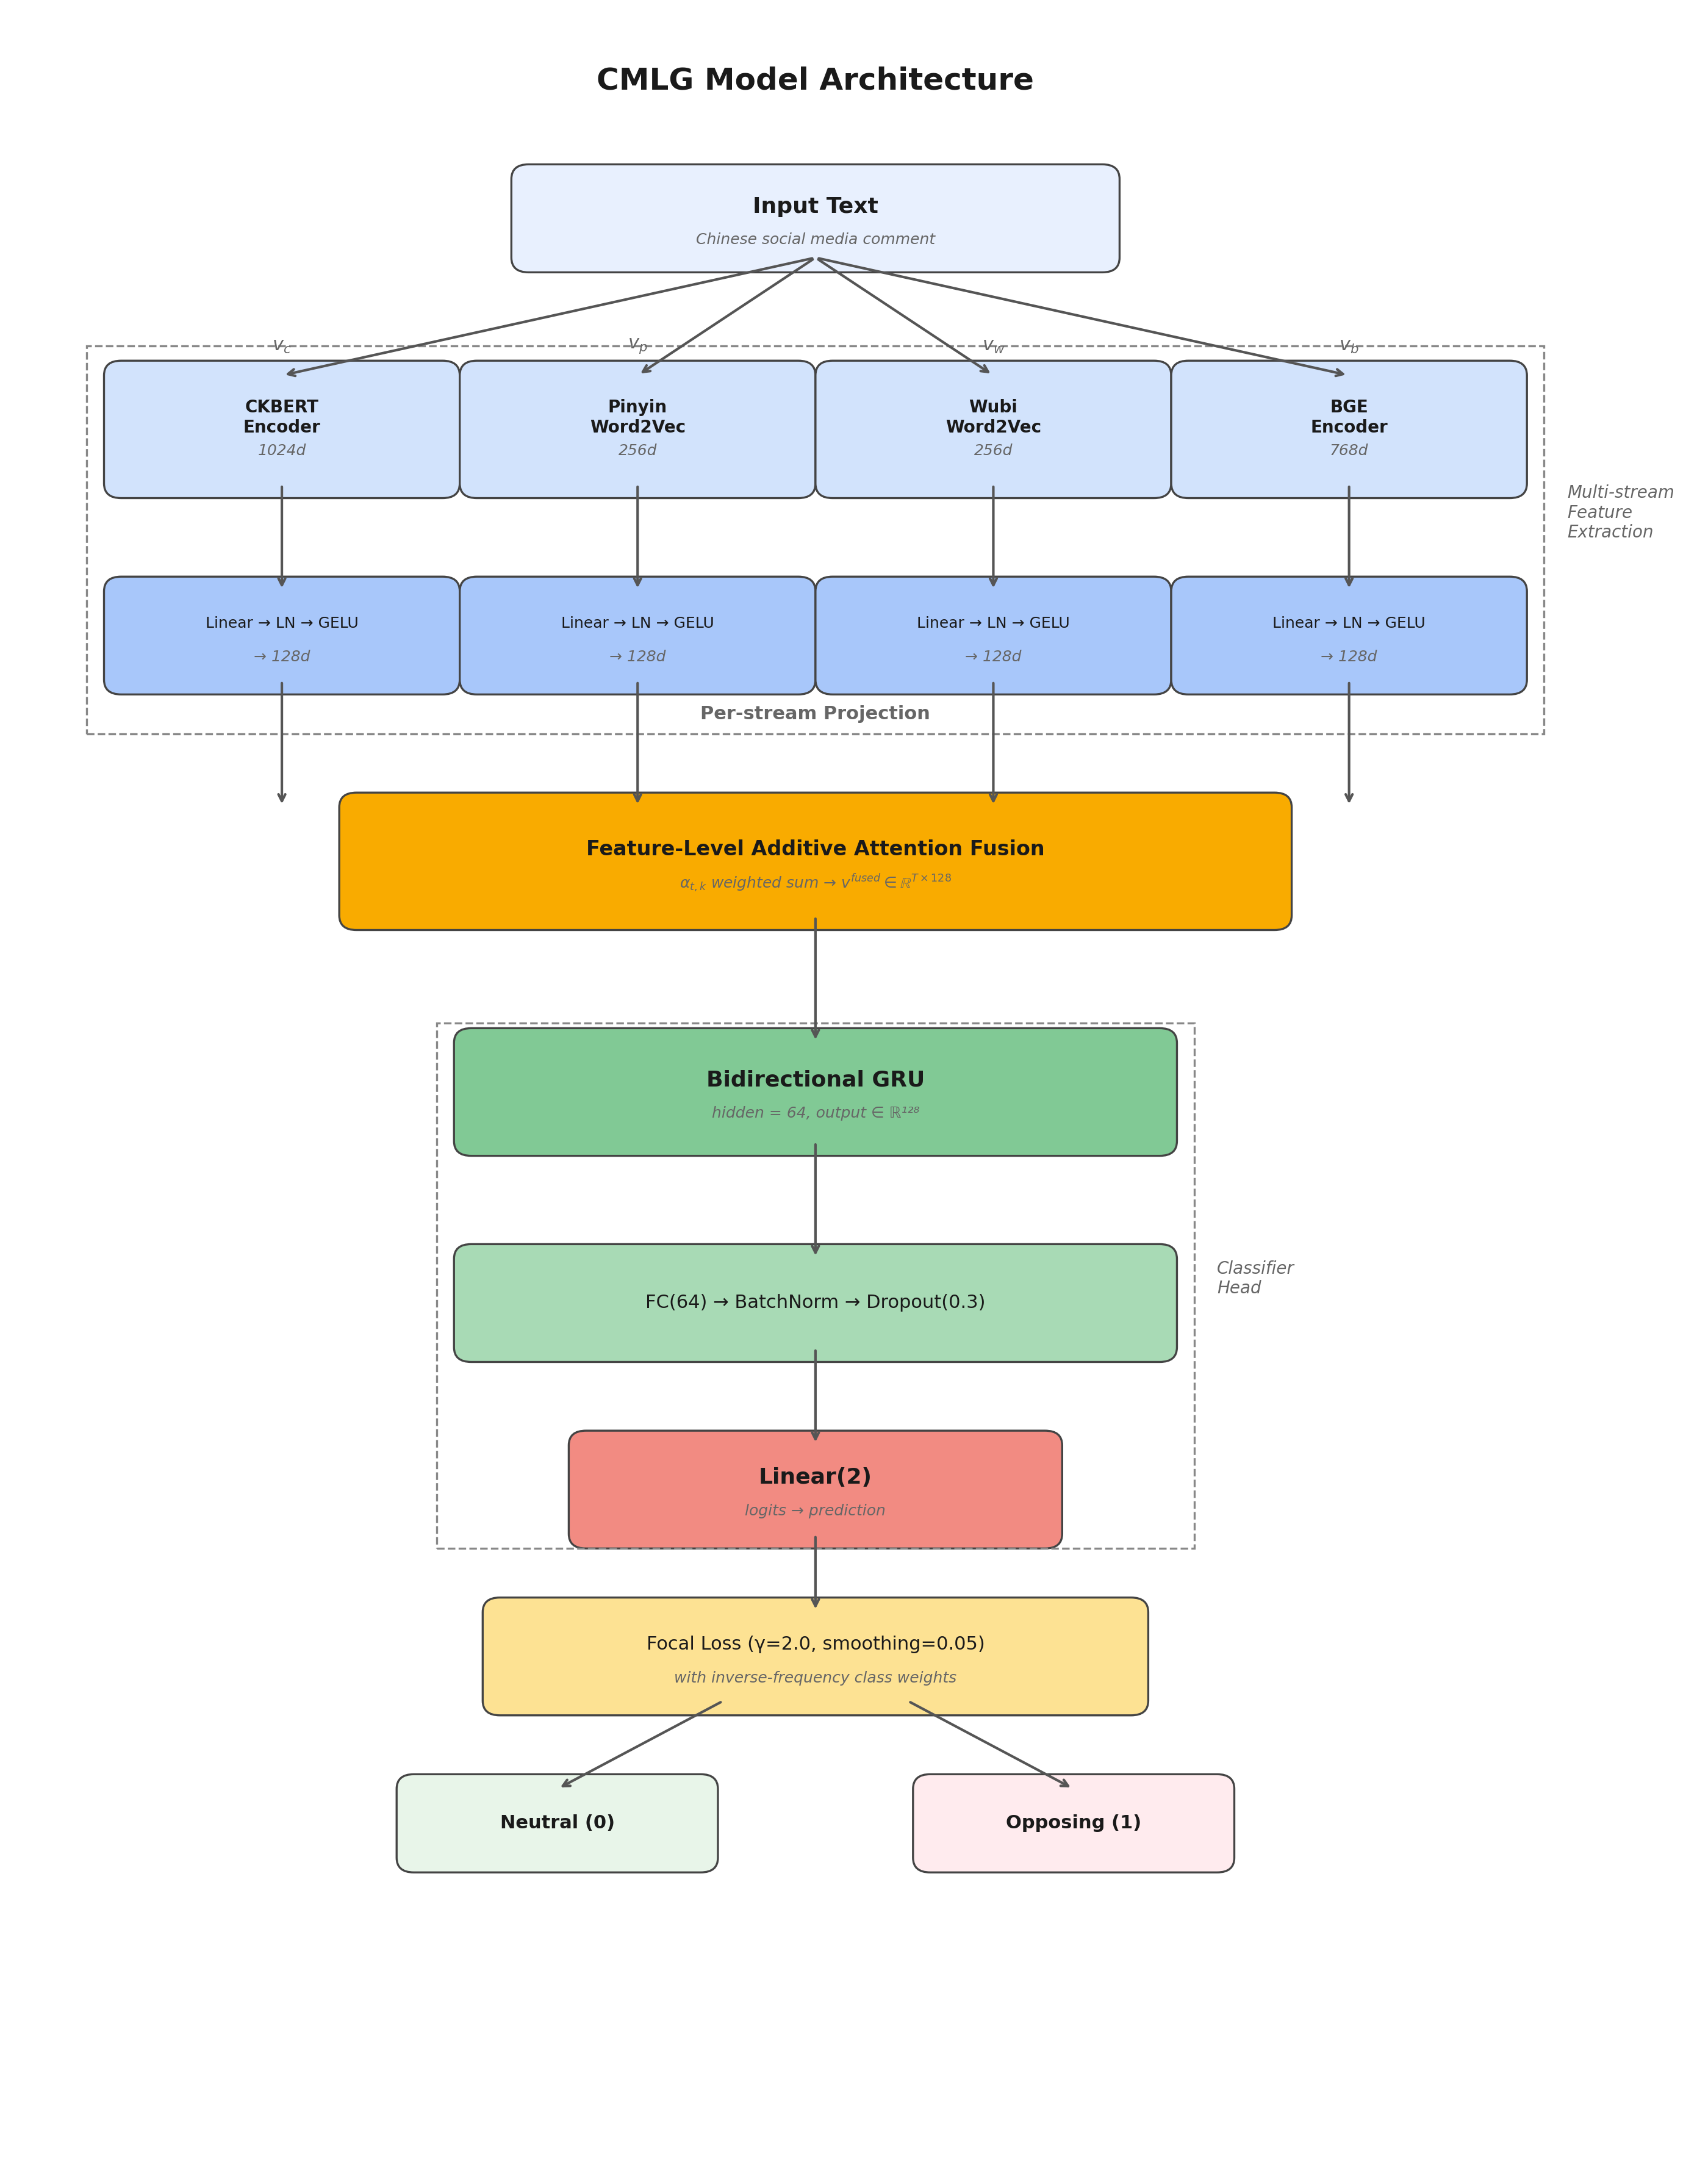
\includegraphics[width=0.78\textwidth]{model_architecture.png}
\caption{CMLG architecture. Four feature streams are projected to 128 dimensions, fused via additive attention, and classified by a Bi-GRU backbone.}
\label{fig:architecture}
\end{figure}

The fused sequence $v^{\mathrm{fused}} \in \mathbb{R}^{T \times 128}$ passes through the following layers. A single-layer bidirectional GRU [21] with hidden size 64 per direction encodes the sequence; the final forward and backward hidden states are concatenated to produce $h_{\mathrm{GRU}} \in \mathbb{R}^{128}$. This vector enters a fully connected block: Linear($128 \to 64$) $\to$ BatchNorm(64) $\to$ ReLU $\to$ Dropout($p = 0.3$) $\to$ Linear($64 \to 2$). The output logits are used directly for prediction (argmax) and for loss computation. The total number of trainable parameters (excluding frozen CKBERT and BGE encoders) is approximately 150K, depending on the number of active streams.

\subsection{Training}
We optimize with AdamW [22] (lr $= 5 \times 10^{-4}$, weight decay $10^{-4}$, gradient clipping at norm 1.0). A ReduceLROnPlateau scheduler halves the learning rate if validation macro F1 does not improve for 7 epochs; training stops early after 20 epochs without improvement. Batch size is 64; maximum sequence length is 512 characters.

For class imbalance we use Focal Loss [11] with focusing parameter $\gamma = 2.0$ and label smoothing $\epsilon = 0.05$:
\[
\mathcal{L}_{\mathrm{focal}} = -\sum_{i} w_{y_i}\,(1 - p_{i,y_i})^{\gamma} \, \log\bigl((1-\epsilon)\,p_{i,y_i} + \epsilon/C\bigr)
\]
where $p_{i,y_i}$ is the predicted probability for the true class of sample $i$, $w_{y_i}$ is the inverse-frequency class weight, and $C=2$ is the number of classes. All results use stratified 5-fold cross-validation.

\section{Experiments and Results}

\subsection{Experimental Setup}
All experiments use a single NVIDIA A100-SXM4-40GB GPU with PyTorch 2.5. Macro F1 under stratified 5-fold cross-validation is the primary metric. We test five feature configurations---\textbf{only\_c} (CKBERT), \textbf{only\_b} (BGE), \textbf{c+b}, \textbf{c+p+w} (CKBERT + pinyin + wubi), and \textbf{c+p+w+b} (all four streams)---to isolate each stream's contribution.

\subsection{Ablation on the Original Dataset}

Table~\ref{tab:original-results} reports the 5-fold results on the original 8{,}969-sample corpus.

\begin{table}[htbp]
\centering
\caption{Ablation results on the original dataset (macro F1 $\pm$ std).}
\label{tab:original-results}
\begin{tabular}{lccccc}
\toprule
Setting & Accuracy & Macro F1 & F1 (Neutral) & F1 (Opposing) \\
\midrule
only\_c   & 0.8203 & 0.7796 $\pm$ 0.0108 & 0.8540 & 0.7136 \\
only\_b   & 0.8132 & 0.7709 $\pm$ 0.0101 & 0.8485 & 0.7020 \\
c+b       & 0.8248 & \textbf{0.7824 $\pm$ 0.0051} & 0.8554 & 0.7177 \\
c+p+w     & 0.8215 & 0.7803 $\pm$ 0.0075 & 0.8539 & 0.7148 \\
c+p+w+b   & 0.8208 & 0.7781 $\pm$ 0.0054 & 0.8531 & 0.7112 \\
\bottomrule
\end{tabular}
\end{table}

All five configurations fall within a 1.2pp band (0.7709--0.7824), with c+b marginally ahead. The minority-class F1 hovers around 0.70--0.72, well below the neutral-class 0.85+, suggesting a shared bottleneck beyond class imbalance. Notably, pinyin and wubi features provide no benefit here---c+p+w trails c+b, and c+p+w+b ranks last. Whether this reflects genuine redundancy or label noise masking orthographic signals is addressed next.

\subsection{Effect of Label Cleaning}

Table~\ref{tab:cleaned-results} reports the same five ablations on both cleaned variants.

\begin{table}[htbp]
\centering
\caption{Ablation results on the cleaned datasets (macro F1 $\pm$ std).}
\label{tab:cleaned-results}
\begin{tabular}{llcccc}
\toprule
Dataset & Setting & Accuracy & Macro F1 & F1 (Neutral) & F1 (Opposing) \\
\midrule
\multirow{5}{*}{\rotatebox{90}{Cleaned-Full}}
& only\_c   & 0.8264 & 0.8206 $\pm$ 0.0080 & 0.8527 & 0.7886 \\
& only\_b   & 0.8100 & 0.8023 $\pm$ 0.0127 & 0.8412 & 0.7635 \\
& c+b       & 0.8295 & 0.8209 $\pm$ 0.0066 & 0.8601 & 0.7817 \\
& c+p+w     & 0.8342 & \textbf{0.8259 $\pm$ 0.0104} & 0.8634 & 0.7885 \\
& c+p+w+b   & 0.8284 & 0.8198 $\pm$ 0.0072 & 0.8587 & 0.7808 \\
\midrule
\multirow{5}{*}{\rotatebox{90}{Cleaned-HC}}
& only\_c   & 0.9020 & 0.8958 $\pm$ 0.0064 & 0.9211 & 0.8704 \\
& only\_b   & 0.8824 & 0.8759 $\pm$ 0.0110 & 0.9043 & 0.8474 \\
& c+b       & 0.9042 & 0.8988 $\pm$ 0.0083 & 0.9221 & 0.8755 \\
& c+p+w     & 0.9068 & \textbf{0.9007 $\pm$ 0.0080} & 0.9253 & 0.8761 \\
& c+p+w+b   & 0.9024 & 0.8963 $\pm$ 0.0104 & 0.9215 & 0.8711 \\
\bottomrule
\end{tabular}
\end{table}

\subsection{Cross-Dataset Comparison}

Table~\ref{tab:cross-dataset} juxtaposes macro F1 and minority-class F1 across datasets.

\begin{table}[htbp]
\centering
\caption{Cross-dataset comparison of macro F1 and opposing-class F1.}
\label{tab:cross-dataset}
\begin{tabular}{lccc|ccc}
\toprule
& \multicolumn{3}{c|}{Macro F1} & \multicolumn{3}{c}{F1 (Opposing)} \\
Setting & Original & Full & HighConf & Original & Full & HighConf \\
\midrule
only\_c   & 0.7796 & 0.8206 & 0.8958 & 0.7171 & 0.7886 & 0.8704 \\
only\_b   & 0.7709 & 0.8023 & 0.8759 & 0.7100 & 0.7635 & 0.8474 \\
c+b       & 0.7824 & 0.8209 & 0.8988 & 0.7267 & 0.7817 & 0.8755 \\
c+p+w     & 0.7803 & \textbf{0.8259} & \textbf{0.9007} & 0.7234 & \textbf{0.7885} & \textbf{0.8761} \\
c+p+w+b   & 0.7781 & 0.8198 & 0.8963 & 0.7181 & 0.7808 & 0.8711 \\
\midrule
Best      & c+b    & c+p+w  & c+p+w  & c+b    & c+p+w / c   & c+p+w \\
$\Delta$ vs Original & --- & +4.4pp & +12.0pp & --- & +6.2pp & +14.9pp \\
\bottomrule
\end{tabular}
\end{table}

Three patterns emerge from Tables~\ref{tab:cleaned-results}--\ref{tab:cross-dataset}. First, the cleaning effect is large: the best macro F1 jumps from 0.7824 (Original) to 0.9007 (Cleaned-HC), a 12pp gain; the minority-class F1 rises even more steeply (+14.9pp), consistent with the smaller class being most affected by noisy labels. Second, a feature-ranking reversal occurs: c+b wins on the noisy original, but c+p+w overtakes it on both cleaned variants, indicating that phonetic and structural cues carry genuine discriminative signal that only becomes learnable under clean supervision. Third, quality dominates quantity---Cleaned-HC retains only 6{,}793 of the original 8{,}969 samples yet substantially outperforms both the full noisy set and Cleaned-Full. The four-stream model (c+p+w+b) consistently underperforms c+p+w, suggesting that the semantic overlap between CKBERT and BGE introduces redundancy that the additive attention mechanism cannot resolve.

\subsection{Baseline Comparison}

We compare CMLG against two baselines under identical evaluation conditions: (i)~SVM with character-level TF-IDF (trigram, 50K features, LinearSVC) and (ii)~BERT-base-chinese with full fine-tuning (5 epochs, lr $2\times10^{-5}$, max length 128). Table~\ref{tab:baselines} reports the results.

\begin{table}[htbp]
\centering
\caption{Comparison with baseline methods across three dataset versions.}
\label{tab:baselines}
\begin{tabular}{llcccc}
\toprule
Dataset & Method & Accuracy & Macro F1 & F1 (Neutral) & F1 (Opposing) \\
\midrule
\multirow{3}{*}{Original}
& SVM + TF-IDF          & 0.8009 & 0.7719 $\pm$ 0.0092 & 0.8532 & 0.6906 \\
& BERT-base-chinese (ft) & 0.8103 & 0.7935 $\pm$ 0.0090 & 0.8517 & 0.7353 \\
& CMLG (c+b)            & 0.8248 & 0.7824 $\pm$ 0.0051 & 0.8554 & 0.7177 \\
\midrule
\multirow{3}{*}{Cleaned-Full}
& SVM + TF-IDF          & 0.8120 & 0.7998 $\pm$ 0.0092 & 0.8492 & 0.7503 \\
& BERT-base-chinese (ft) & 0.8455 & \textbf{0.8399 $\pm$ 0.0100} & 0.8696 & 0.8102 \\
& CMLG (c+p+w)          & 0.8342 & 0.8259 $\pm$ 0.0104 & 0.8634 & 0.7885 \\
\midrule
\multirow{3}{*}{Cleaned-HC}
& SVM + TF-IDF          & 0.8762 & 0.8679 $\pm$ 0.0043 & 0.9010 & 0.8347 \\
& BERT-base-chinese (ft) & 0.9182 & \textbf{0.9128 $\pm$ 0.0039} & 0.9344 & 0.8911 \\
& CMLG (c+p+w)          & 0.9068 & 0.9007 $\pm$ 0.0080 & 0.9253 & 0.8761 \\
\bottomrule
\end{tabular}
\end{table}

BERT fine-tuning outperforms CMLG by 1.1--1.4pp in macro F1 across all datasets. This is expected: BERT-ft updates all 110M+ transformer parameters end-to-end, whereas CMLG freezes its pretrained encoders and trains only the projection, attention, and GRU layers ($\sim$150K parameters). SVM trails both neural methods substantially. The cleaning effect is consistent across all three methods (9--14pp gains from Original to Cleaned-HC), confirming that annotation quality, rather than model choice, is the primary constraint.

\section{Discussion}

\subsection{Orthographic Features and Label Quality}
The feature-ranking reversal between noisy and clean data is the central empirical finding. On the original labels, pinyin and wubi features add nothing; on cleaned labels, c+p+w consistently leads. This resolves an apparent contradiction with Ma et al.\ [9], who reported gains from character-form features on SWSR: the discrepancy likely reflects differences in noise levels between their processing and ours. Mechanistically, the attention module learns to up-weight whichever stream is most informative at each character position; under noisy supervision, these weights become unreliable and the fusion degrades toward uniform averaging, erasing the advantage of fine-grained orthographic cues.

\subsection{Why BERT Fine-tuning Outperforms CMLG}
BERT-ft updates 110M+ parameters end-to-end, while CMLG trains only $\sim$150K parameters atop frozen encoders---the 1--1.4pp gap is modest given this asymmetry. The trade-off is interpretability: CMLG's modular architecture makes it possible to isolate which feature streams contribute and how their utility depends on label quality, an analysis that monolithic fine-tuning does not support. The finding that orthographic features shift from useless to most valuable after cleaning would not have been discoverable from BERT-ft experiments alone.

\subsection{Annotation Quality as the Dominant Factor}
The 12pp macro F1 gain from label cleaning---observed across all three methods---dwarfs anything achievable by changing features or models on the noisy data (total spread: 1.2pp). This is consistent with the label-noise literature [19,20] and suggests that for this task, improvements in annotation quality yield higher returns than architectural advances. The quantity--quality trade-off reinforces this point: discarding 24\% of the corpus through unanimous-agreement filtering produces a far better training signal than retaining all noisy samples.

\subsection{Limitations}
The binary formulation collapses directional stance, limiting downstream utility. The three LLMs share similar pretraining paradigms and may make correlated errors on genuinely ambiguous samples, introducing systematic bias into the cleaned labels. All data come from SWSR; cross-platform generalization is untested. The consistent underperformance of c+p+w+b relative to c+p+w indicates that additive attention is insufficient for resolving high inter-stream redundancy; more expressive fusion mechanisms (e.g., cross-attention or gating) may be needed.

\section{Conclusion}
We proposed CMLG, a multi-stream model that fuses CKBERT, BGE, pinyin, and wubi features through learnable attention for gender-antagonistic discourse detection in Chinese social media, and coupled it with an LLM-based label cleaning pipeline.

Experiments across three dataset versions, five feature configurations, and two baselines yield three findings. First, label cleaning raises macro F1 by 9--14pp for every method tested---including SVM and BERT---establishing annotation quality as the dominant factor. Second, Chinese orthographic features (pinyin, wubi) are ineffective under noisy labels but become the strongest feature configuration after cleaning, demonstrating that annotation quality gates the learnability of fine-grained linguistic cues. Third, retaining only unanimously agreed samples outperforms the full noisy corpus despite a 24\% reduction in data volume.

Future work will extend the framework to directional stance classification, evaluate cross-platform generalization, and explore more expressive fusion mechanisms.

\appendix
\section{LLM Cleaning Prompt}
\label{app:prompt}
The following Chinese prompt was sent identically to each of the three LLMs. Input texts exceeding 500 characters were truncated before querying.

\begin{quote}
\small
你是一个中文社交媒体文本分类专家，专门识别性别对立言论。

分类标准：

- 性别对立言论（标签1）：针对特定性别群体的贬低、攻击、歧视、污名化、刻板印象强化、挑拨性别矛盾的言论。包括但不限于：使用性别歧视性称呼（如"婚驴""舔狗""小仙女"等讽刺性称呼）、将负面特征归因于某一性别、煽动性别对立情绪。

- 中立言论（标签0）：不包含上述内容的普通评论，即使话题涉及性别议题，只要表达方式客观理性、不带攻击性，也属于中立。

注意：

- 仅根据文本本身判断，不要推测发言者意图

- 反讽、阴阳怪气的性别攻击也算对立言论

- 讨论性别议题但不带攻击性的属于中立

请判断以下中文社交媒体评论是否为性别对立言论。

评论：\{text\}

请只回复一个数字：1（性别对立）或 0（中立）。
\end{quote}

\section*{References}
\begin{enumerate}
\item X. Luo, B. Liang, Q. Wang, J. Li, E. Cambria, X. Zhang, Y. He, M. Yang, and R. Xu, ``A literature survey on multimodal and multilingual sexism detection,'' \textit{IEEE Trans. Comput. Social Syst.}, vol.~12, no.~5, pp.~3709--3727, 2025, doi: 10.1109/TCSS.2025.3561921.

\item B. Qin and X. Wang, ``The impact of gender antagonism online public opinion on contemporary college students and countermeasures,'' \textit{J. Langfang Norm. Univ. (Soc. Sci. Ed.)}, vol.~40, no.~2, pp.~95--102, 2024, doi: 10.16124/j.cnki.cn13-1390/c.2024.02.002.

\item L. Fontanella, B. Chulvi, E. Ignazzi, A. Sarra, and A. Tontodimamma, ``How do we study misogyny in the digital age? A systematic literature review using a computational linguistic approach,'' \textit{Humanit. Soc. Sci. Commun.}, vol.~11, no.~1, p.~478, Apr. 2024, doi: 10.1057/s41599-024-02978-7.

\item B. G. Gutam, S. C. D, J. N. Kumar, S. D. Babu, J. S. Babu, and M. S. Kumar, ``A machine learning and community-driven approach for feminist cyber resistance framework to mitigate online gender-based violence,'' in \textit{Proc. 4th OPJU Int. Technol. Conf. (OTCON)}, 2025, pp.~1--5, doi: 10.1109/OTCON65728.2025.11070859.

\item A. Singh, D. Sharma, and V. K. Singh, ``Misogynistic attitude detection in YouTube comments and replies: A high-quality dataset and algorithmic models,'' \textit{Comput. Speech Lang.}, vol.~89, Art. no. 101682, 2025, doi: 10.1016/j.csl.2024.101682.

\item M. N. Vivekananda, V. V. Malgi, and P. A. Shidlyali, ``Integrating transformers and hybrid machine learning models for automated sexism detection in online discourse,'' in \textit{Proc. Int. Conf. AMATHE}, 2025, pp.~1--6, doi: 10.1109/amathe65477.2025.11081244.

\item A. Mohasseb, E. Amer, F. Chiroma, and A. Tranchese, ``Leveraging advanced NLP techniques and data augmentation to enhance online misogyny detection,'' \textit{Appl. Sci.}, vol.~15, no.~2, Art. no. 856, Jan. 2025, doi: 10.3390/app15020856.

\item A. Jiang, X. Yang, Y. Liu, and A. Zubiaga, ``SWSR: A Chinese dataset and lexicon for online sexism detection,'' \textit{Online Social Netw. Media}, vol.~27, p.~100182, 2022, doi: 10.1016/j.osnem.2021.100182.

\item Z. Ma, S. Zhang, Y. Liu, and G. Zhang, ``A gender-opposition speech recognition method integrating multi-features and expression emotion dictionary,'' \textit{J. Data Acquis. Process.}, vol.~39, no.~3, 2024, doi: 10.16337/j.1004-9037.2024.03.017.

\item T. Zhang, J. Dong, J. Wang, C. Wang, A. Wang, Y. Liu, J. Huang, Y. Li, and X. He, ``Revisiting and advancing Chinese natural language understanding with accelerated heterogeneous knowledge pre-training,'' in \textit{Proc. EMNLP (Industry Track)}, 2022, pp.~1634--1645.

\item T.-Y. Lin, P. Goyal, R. Girshick, K. He, and P. Doll\'{a}r, ``Focal loss for dense object detection,'' in \textit{Proc. IEEE Int. Conf. Comput. Vis. (ICCV)}, 2017, pp.~2980--2988, doi: 10.1109/ICCV.2017.324.

\item J. Devlin, M.-W. Chang, K. Lee, and K. Toutanova, ``BERT: Pre-training of deep bidirectional transformers for language understanding,'' in \textit{Proc. NAACL-HLT}, 2019, pp.~4171--4186.

\item S. Xiao, Z. Liu, P. Zhang, and N. Muennighoff, ``C-Pack: Packaged resources to advance general Chinese embedding,'' in \textit{Proc. ACL}, 2024, pp.~2523--2535, doi: 10.18653/v1/2024.acl-long.138.

\item T. Mikolov, K. Chen, G. Corrado, and J. Dean, ``Efficient estimation of word representations in vector space,'' in \textit{Proc. ICLR Workshop}, 2013, arXiv: 1301.3781.

\item D. Bahdanau, K. Cho, and Y. Bengio, ``Neural machine translation by jointly learning to align and translate,'' in \textit{Proc. ICLR}, 2015, arXiv: 1409.0473.

\item P. Fortuna and S. Nunes, ``A survey on automatic detection of hate speech in text,'' \textit{ACM Comput. Surv.}, vol.~51, no.~4, Art. no. 85, Jul. 2018, doi: 10.1145/3232676.

\item T. Davidson, D. Warmsley, M. Macy, and I. Weber, ``Automated hate speech detection and the problem of offensive language,'' in \textit{Proc. ICWSM}, 2017, pp.~512--515.

\item C. Sun, X. Qiu, Y. Xu, and X. Huang, ``How to fine-tune BERT for text classification?'' in \textit{Chinese Computational Linguistics (CCL)}, Lecture Notes in Computer Science, vol.~11856, 2019, pp.~194--206, doi: 10.1007/978-3-030-32381-3\_16.

\item B. Fr\'{e}nay and M. Verleysen, ``Classification in the presence of label noise: A survey,'' \textit{IEEE Trans. Neural Netw. Learn. Syst.}, vol.~25, no.~5, pp.~845--869, 2014, doi: 10.1109/TNNLS.2013.2292894.

\item H. Song, M. Kim, D. Park, Y. Shin, and J.-G. Lee, ``Learning from noisy labels with deep neural networks: A survey,'' \textit{IEEE Trans. Neural Netw. Learn. Syst.}, vol.~34, no.~11, pp.~8135--8153, 2023, doi: 10.1109/TNNLS.2022.3152527.

\item K. Cho, B. van Merri\"{e}nboer, C. Gulcehre, D. Bahdanau, F. Bougares, H. Schwenk, and Y. Bengio, ``Learning phrase representations using RNN encoder--decoder for statistical machine translation,'' in \textit{Proc. EMNLP}, 2014, pp.~1724--1734, doi: 10.3115/v1/D14-1179.

\item I. Loshchilov and F. Hutter, ``Decoupled weight decay regularization,'' in \textit{Proc. ICLR}, 2019, arXiv: 1711.05101.

\end{enumerate}

\end{document}
